\documentclass[10pt]{article}
\usepackage[T1]{fontenc}

% Document Details
\newcommand{\CLASS}{AMATH 586}
\newcommand{\assigmentnum}{Assignment 4}

\usepackage[margin = 1.15in, top = 1.25in, bottom = 1.in]{geometry}

\usepackage{titling}
\setlength{\droptitle}{-6em}   % This is your set screw
\date{}
\renewcommand{\maketitle}{
	\clearpage
	\begingroup  
	\centering
	\LARGE \sffamily\textbf{\CLASS} \Large \assigmentnum\\[.8em]
	\large Tyler Chen\\[1em]
	\endgroup
	\thispagestyle{empty}
}
 % Title Styling
\usepackage{tocloft}
\renewcommand{\cfttoctitlefont}{\Large\sffamily\bfseries}
\renewcommand{\cftsecfont}{\normalfont\sffamily\bfseries}
\renewcommand{\cftsubsecfont}{\normalfont\sffamily}
\renewcommand{\cftsubsubsecfont}{\normalfont\sffamily}

\makeatletter
\let\oldl@section\l@section
\def\l@section#1#2{\oldl@section{#1}{\sffamily\bfseries#2}}

\let\oldl@subsection\l@subsection
\def\l@subsection#1#2{\oldl@subsection{#1}{\sffamily#2}}

\let\oldl@subsubsection\l@subsubsection
\def\l@subsubsection#1#2{\oldl@subsubsection{#1}{\sffamily#2}}
 % General Styling


\usepackage{enumitem}

% Figures
\usepackage{subcaption}

% TikZ and Graphics
\usepackage{tikz, pgfplots}
\pgfplotsset{compat=1.12}
\usetikzlibrary{patterns,arrows}
\usepgfplotslibrary{fillbetween}

\usepackage{pdfpages}
\usepackage{adjustbox}

\usepackage{lscape}
\usepackage{titling}
\usepackage[]{hyperref}


% Header Styling
\usepackage{fancyhdr}
\pagestyle{fancy}
\lhead{\sffamily \CLASS}
\rhead{\sffamily Chen \textbf{\thepage}}
\cfoot{}

% Paragraph Styling
\setlength{\columnsep}{1cm}
\setlength{\parindent}{0pt}
\setlength{\parskip}{5pt}
\renewcommand{\baselinestretch}{1}

% TOC Styling
\usepackage{tocloft}
\iffalse
\renewcommand{\cftsecleader}{\cftdotfill{\cftdotsep}}

\renewcommand\cftchapafterpnum{\vskip6pt}
\renewcommand\cftsecafterpnum{\vskip10pt}
\renewcommand\cftsubsecafterpnum{\vskip6pt}

% Adjust sectional unit title fonts in ToC
\renewcommand{\cftchapfont}{\sffamily}
\renewcommand{\cftsecfont}{\bfseries\sffamily}
\renewcommand{\cftsecnumwidth}{2em}
\renewcommand{\cftsubsecfont}{\sffamily}
\renewcommand{\cfttoctitlefont}{\hfill\bfseries\sffamily\MakeUppercase}
\renewcommand{\cftaftertoctitle}{\hfill}

\renewcommand{\cftchappagefont}{\sffamily}
\renewcommand{\cftsecpagefont}{\bfseries\sffamily}
\renewcommand{\cftsubsecpagefont}{\sffamily}
\fi
 % General Styling
% Code Display Setup
\usepackage{listings,lstautogobble}
\usepackage{lipsum}
\usepackage{courier}
\usepackage{catchfilebetweentags}

\lstset{
	basicstyle=\small\ttfamily,
	breaklines=true, 
	frame = single,
	rangeprefix=,
	rangesuffix=,
	includerangemarker=false,
	autogobble = true
}


\usepackage{algorithmicx}
\usepackage{algpseudocode}

\newcommand{\To}{\textbf{to}~}
\newcommand{\DownTo}{\textbf{downto}~}
\renewcommand{\algorithmicdo}{\hspace{-.2em}\textbf{:}}
 % Code Display Setup
% AMS MATH Styling
\usepackage{amsmath, amssymb}
\newcommand{\qed}{\hfill\(\square\)}

%\newtheorem*{lemma}{Lemma} 
%\newtheorem*{theorem}{Theorem}
%\newtheorem*{definition}{Definition}
%\newtheorem*{prop}{Proposition}
%\renewenvironment{proof}{{\bfseries Proof.}}{}


% mathcal
\newcommand{\cA}{\ensuremath{\mathcal{A}}}
\newcommand{\cB}{\ensuremath{\mathcal{B}}}
\newcommand{\cC}{\ensuremath{\mathcal{C}}}
\newcommand{\cD}{\ensuremath{\mathcal{D}}}
\newcommand{\cE}{\ensuremath{\mathcal{E}}}
\newcommand{\cF}{\ensuremath{\mathcal{F}}}
\newcommand{\cG}{\ensuremath{\mathcal{G}}}
\newcommand{\cH}{\ensuremath{\mathcal{H}}}
\newcommand{\cI}{\ensuremath{\mathcal{I}}}
\newcommand{\cJ}{\ensuremath{\mathcal{J}}}
\newcommand{\cK}{\ensuremath{\mathcal{K}}}
\newcommand{\cL}{\ensuremath{\mathcal{L}}}
\newcommand{\cM}{\ensuremath{\mathcal{M}}}
\newcommand{\cN}{\ensuremath{\mathcal{N}}}
\newcommand{\cO}{\ensuremath{\mathcal{O}}}
\newcommand{\cP}{\ensuremath{\mathcal{P}}}
\newcommand{\cQ}{\ensuremath{\mathcal{Q}}}
\newcommand{\cR}{\ensuremath{\mathcal{R}}}
\newcommand{\cS}{\ensuremath{\mathcal{S}}}
\newcommand{\cT}{\ensuremath{\mathcal{T}}}
\newcommand{\cU}{\ensuremath{\mathcal{U}}}
\newcommand{\cV}{\ensuremath{\mathcal{V}}}
\newcommand{\cW}{\ensuremath{\mathcal{W}}}
\newcommand{\cX}{\ensuremath{\mathcal{X}}}
\newcommand{\cY}{\ensuremath{\mathcal{Y}}}
\newcommand{\cZ}{\ensuremath{\mathcal{Z}}}

% mathbb
\usepackage{bbm}
\newcommand{\bOne}{\ensuremath{\mathbbm{1}}}

\newcommand{\bA}{\ensuremath{\mathbb{A}}}
\newcommand{\bB}{\ensuremath{\mathbb{B}}}
\newcommand{\bC}{\ensuremath{\mathbb{C}}}
\newcommand{\bD}{\ensuremath{\mathbb{D}}}
\newcommand{\bE}{\ensuremath{\mathbb{E}}}
\newcommand{\bF}{\ensuremath{\mathbb{F}}}
\newcommand{\bG}{\ensuremath{\mathbb{G}}}
\newcommand{\bH}{\ensuremath{\mathbb{H}}}
\newcommand{\bI}{\ensuremath{\mathbb{I}}}
\newcommand{\bJ}{\ensuremath{\mathbb{J}}}
\newcommand{\bK}{\ensuremath{\mathbb{K}}}
\newcommand{\bL}{\ensuremath{\mathbb{L}}}
\newcommand{\bM}{\ensuremath{\mathbb{M}}}
\newcommand{\bN}{\ensuremath{\mathbb{N}}}
\newcommand{\bO}{\ensuremath{\mathbb{O}}}
\newcommand{\bP}{\ensuremath{\mathbb{P}}}
\newcommand{\bQ}{\ensuremath{\mathbb{Q}}}
\newcommand{\bR}{\ensuremath{\mathbb{R}}}
\newcommand{\bS}{\ensuremath{\mathbb{S}}}
\newcommand{\bT}{\ensuremath{\mathbb{T}}}
\newcommand{\bU}{\ensuremath{\mathbb{U}}}
\newcommand{\bV}{\ensuremath{\mathbb{V}}}
\newcommand{\bW}{\ensuremath{\mathbb{W}}}
\newcommand{\bX}{\ensuremath{\mathbb{X}}}
\newcommand{\bY}{\ensuremath{\mathbb{Y}}}
\newcommand{\bZ}{\ensuremath{\mathbb{Z}}}

% alternative mathbb
\newcommand{\NN}{\ensuremath{\mathbb{N}}}
\newcommand{\RR}{\ensuremath{\mathbb{R}}}
\newcommand{\CC}{\ensuremath{\mathbb{C}}}
\newcommand{\ZZ}{\ensuremath{\mathbb{Z}}}
\newcommand{\EE}{\ensuremath{\mathbb{E}}}
\newcommand{\PP}{\ensuremath{\mathbb{P}}}
\newcommand{\VV}{\ensuremath{\mathbb{V}}}
\newcommand{\cov}{\ensuremath{\text{Co}\VV}}
% Math Commands

\newcommand{\st}{~\big|~}
\newcommand{\stt}{\text{ st. }}
\newcommand{\ift}{\text{ if }}
\newcommand{\thent}{\text{ then }}
\newcommand{\owt}{\text{ otherwise }}

\newcommand{\norm}[1]{\left\lVert#1\right\rVert}
\newcommand{\snorm}[1]{\lVert#1\rVert}
\newcommand{\ip}[1]{\ensuremath{\left\langle #1 \right\rangle}}
\newcommand{\pp}[3][]{\frac{\partial^{#1}#2}{\partial #3^{#1}}}
\newcommand{\dd}[3][]{\frac{\d^{#1}#2}{\d #3^{#1}}}
\renewcommand{\d}{\ensuremath{\mathrm{d}}}

\newcommand{\indep}{\rotatebox[origin=c]{90}{$\models$}}




 % Math shortcuts
% Problem
\usepackage{floatrow}

\newenvironment{problem}[1][]
{\pagebreak
\noindent\rule{\textwidth}{1pt}\vspace{0.25em}
{\sffamily \textbf{#1}}
\par
}
{\par\vspace{-0.5em}\noindent\rule{\textwidth}{1pt}}

\newenvironment{solution}[1][]
{{\sffamily \textbf{#1}}
\par
}
{}

 % Problem Environment

\newcommand{\note}[1]{\textcolor{red}{\textbf{Note:} #1}}

\hypersetup{
   colorlinks=true,       % false: boxed links; true: colored links
   linkcolor=violet,          % color of internal links (change box color with linkbordercolor)
   citecolor=green,        % color of links to bibliography
   filecolor=magenta,      % color of file links
   urlcolor=cyan           % color of external links
}


\begin{document}
\maketitle


\begin{problem}[Problem 1]
Consider the following method for solving the heat equation \(u_t = u_{xx}\):
\[
U_j^{n+2} = U_j^n + \frac{2k}{h^2} ( U_{j-1}^{n+1} - 2 U_j^{n+1} + U_{j+1}^{n+1} ) .
\]
\begin{enumerate}[label=(\alph*)]
\item Determine the formal order of accuracy of this method (in both space and time) based on computing the local truncation error.
\item Suppose we take \(k = \alpha h^2\) for some fixed \(\alpha > 0\) and refine the grid.  Show that this method fails to be Lax-Richtmyer stable for any choice of \(\alpha\).

Do this in two ways:
\begin{itemize}
\item Consider the MOL interpretation and the stability region of the time-discretization being used.
\item Use von Neumann analysis and solve a quadratic equation for \(g( \xi )\).
\end{itemize}
\item What if we take \(k = \alpha h^3\) for some fixed \(\alpha > 0\) and refine the grid.  Would this method be stable?  Justify your answer.
\end{enumerate}
\end{problem}

\begin{solution}[Solution]

\begin{enumerate}[label=(\alph*)]
    \item We have,
    \begin{align*}
        \dfrac{1}{2k}(u(x,t+2k) - u(x,t)) = \dfrac{1}{h^2} \left( u(x-h,t+k) - 2u(x,t+k) + u(x+h,t+k) \right) + \tau(x,t)
    \end{align*}

    Therefore, by the definition of local truncation error,
    \begin{align*}
        \tau(x,t) =\dfrac{1}{2k} \left( u(x,t+2k) - u(x,t) \right) - \dfrac{1}{h^2} \left( u(x-h,t+k) - 2u(x,t+k) + u(x+h,t+k) \right)
    \end{align*}

    Using Mathematica,
    \begin{lstlisting}
        U[dx_, dt_] := Normal[Series[u[dx h z + x, dt k z + t], {z, 0, 4}]] /. {z -> 1}
        LTE = FullSimplify
                [1/(2k) (U[0,2]-U[0,0])-1/h^2 (U[-1,1]-2U[0,1]+U[1,1]),
                Assumptions->{
                    D[u[x,t],t]==D[u[x,t],{x,2}],
                    D[u[x,t],{t,2}]==D[u[x,t],t,{x,2}],
                    D[u[x,t],{t,3}]==D[u[x,t],{x,2},{t,2}]
                }
              ]
    \end{lstlisting}
    This gives,
    \begin{align*}
        \tau(x,t) = k^2 \left( \dfrac{1}{6}u_{ttt} \right) - h^2 \left( \dfrac{1}{12}u_{tt} \right) + \cO(k^3) + \cO(h^3)
    \end{align*}

    \item
    We can view the above method as the midpoint method applied to the system,
    \begin{align*}
        U_j'(t) = \dfrac{1}{h^2}(U_{j-1}(t) - 2 U_{j}(t) + U_{j+1}(t))
    \end{align*}

    In matrix notation,
    \begin{align*}
        U' = AU,
        &&A = \dfrac{1}{h^2}\left[\begin{array}{ccccc}-2 & 1 \\
        1 & \ddots & \ddots \\
        & \ddots \end{array}\right]
    \end{align*}

    Note that \( A \) is normal as it is symmetric. Then, for stability of the midpoints method we require that for all eigenvalues \( \lambda \) of \( A \),
    \begin{align*}
        |\operatorname{Im}(1+2k\lambda)|\leq 1 && \operatorname{Re}(1+2k\lambda) = 0
    \end{align*}

    The eigenvalues of \( A \) are,
    \begin{align*}
        \lambda_p = \dfrac{2}{h^2}(\cos(p\pi h)-1), && p=1,2,\ldots, m
    \end{align*}

    Then, taking \( k = \alpha h^2 \) for some \( \alpha > 0 \),
    \begin{align*}
        k\lambda_p = 2\alpha(\cos(p\pi h)-1)
    \end{align*}

    Clearly \( \lambda_p \) are all real and distinct. Therefore \( 1 + 2k\lambda_p \) cannot have zero real part for all \( \lambda_p \).  Therefore this method is not stable for any \( \alpha \). \qed

    Set \( U_j^n = e^{ijh\xi} \). Then, \( U_j^{n+1} = g(\xi)e^{ijh\xi} \) and \( U_j^{n+2} = g(\xi)^2e^{ijh\xi} \). Inserting these into method we have,
    \begin{align*}
        g(\xi)^2e^{ijh\xi} = e^{ijh\xi} + \dfrac{2k}{h^2}\left( g(\xi)e^{i(j-1)h\xi} - 2g(\xi)e^{ijh\xi} + g(\xi)e^{i(j+1)h\xi} \right)
    \end{align*}

    Dividing through by \( e^{ijh\xi} \), using the identity \( e^{-ih\xi} + e^{ih\xi} = 2\cos(h\xi) \), and moving everything to the left gives,
    \begin{align*}
        0 &= g(\xi)^2 - \dfrac{2k}{h^2}\left( e^{-ih\xi} - 2 + e^{ih\xi} \right)g(\xi) - 1
        \\&= g(\xi)^2 - \dfrac{4k}{h^2}(\cos(h\xi)-1)g(\xi) - 1
    \end{align*}

    This is a quadratic in \( g(\xi) \) with solutions,
    \begin{align*}
        g(\xi) &= \dfrac{2k/h^2(\cos(h\xi)-1) \pm \sqrt{(4k/h^2(\cos(h\xi)-1))^2-4(1)(-1)}}{2}
        \\&= \dfrac{k}{h^2}(\cos(h\xi)-1) \pm \sqrt{\dfrac{2^2k^2}{h^4}(\cos(h\xi)-1)^2+1}
    \end{align*}

    %For convenience write \( a = 2k/h^2(\cos(h\xi)-1) \).
    Note that \( \sqrt{a^2+1} > 1 \) so that if \( a < 0 \), \( a/2 - \sqrt{a^2+1} < -1 \).

    Suppose \( k = \alpha h^2 \) for some \( \alpha > 0 \). Then \( a = 2\alpha(\cos(h\xi)-1) \). Clearly for sufficiently small \( h \) and any real \( \xi \) we have \( \cos(h\xi) \to 1^- \) so \( a<0 \). Thus,
    \begin{align*}
        |g(\xi)| = \left|\alpha(\cos(h\xi)-1) - \sqrt{2^2\alpha^2 (\cos(h\xi)-1)^2+1}\right| > 1
    \end{align*}

    Therefore there are values of \( \xi \) for which \( |g(\xi)| > 1 \). This proves the method is not stable when \( k = \alpha h^2 \) as \( h\to 0 \). \qed

    \item
    If we take \( k = \alpha h^3 \) then \( a = h\alpha(\cos(h\xi)-1) \). Again as \( h\to 0 \) we have \( a < 0 \).
    Therefore there are values of \( \xi \) for which \( |g(\xi)| > 1 \). This proves the method is not stable for  \( k = \alpha h^3 \) as \( h\to 0 \). \qed


\end{enumerate}


\end{solution}

\begin{problem}[Problem 2]
Consider the PDE
\[
u_t = \kappa u_{xx} - \gamma u ,
\]
which models diffusion combined with decay provided \(\kappa > 0\) and \(\gamma > 0\).
Consider methods of the form
\[
U_j^{n+1} = U_j^n + \frac{k \kappa}{2 h^2} [ U_{j-1}^n - 2 U_j^n + U_{j+1}^n + U_{j-1}^{n+1} -
2 U_j^{n+1} + U_{j+1}^{n+1} ] - k \gamma [ (1 - \theta ) U_j^n + \theta U_j^{n+1} ] ,
\]
where \(\theta\) is a parameter.  In particular, if \(\theta = 1/2\) then the decay term is modeled with the same centered-in-time approach as the diffusion term and the method can be obtained by applying the trapezoidal method to the MOL formulation of the PDE.  If \(\theta = 0\) then the decay term is handled explicitly.  For more general reaction-diffusion equations it may be advantageous to handle the reaction terms explicitly since these terms are generally nonlinear, so making them implicit would require solving nonlinear systems at each time step (whereas handling the diffusion term implicitly only gives a linear system to solve at each time step).
\begin{enumerate}[label=(\alph*)]
\item
By computing the local truncation error, show that this method is \(O( k^p + h^2 )\) accurate,
where \(p = 2\) if \(\theta = 1/2\) and \(p = 1\) otherwise.
\item
Using von Neumann analysis, show that this method is unconditionally stable if \(\theta \geq 1/2\).
\item
Show that if \(\theta = 0\) then the method is stable provided \(k \leq 2/ \gamma\), independent of \(h\).
\end{enumerate}
\end{problem}

\begin{solution}[Solution]

\begin{enumerate}[label=(\alph*)]
    \item We have,
    \begin{align*}
        \dfrac{1}{k}(u(x,t+k) - u(x,t)) &= \dfrac{\kappa}{2h^2} ( u(x-h,t) - 2u(x+h,t) + u(x-h,t) + u(x-h,t+k) - 2u(x,t+k)
        \\& \hspace{4em} + u(x+h,t+k) ) - \gamma((1-\theta)u(x,t) + \theta u(x,t+k) ) + \tau(x,t)
    \end{align*}

    Therefore, by the definition of local truncation error,
    \begin{align*}
        \tau(x,t) &= \dfrac{1}{k}(u(x,t+k) - u(x,t)) -  \dfrac{\kappa}{2h^2} ( u(x-h,t) - 2u(x+h,t) + u(x-h,t+k)
        \\& \hspace{4em} + u(x-h,t+k)  - 2u(x,t+k) + u(x+h,t+k) ) + \gamma((1-\theta)u(x,t) + \theta u(x,t+k) )
    \end{align*}

    Using Mathematica,
    \begin{lstlisting}
    U[dx_, dt_] := Normal[Series[u[dx h z + x, dt k z + t], {z, 0, 4}]] /. {z -> 1}
    LTE = Collect[FullSimplify[
            1/k (U[0,1]-U[0,0])-\[Kappa]/(2h^2) (U[-1,0]-2U[0,0]+U[1,0]+U[-1,1]-2U[0,1]+U[1,1])+ \[Gamma]((1-\[Theta])U[0,0]+\[Theta] U[0,1]),
            Assumptions->{
                D[u[x,t],t]==\[Kappa] D[u[x,t],{x,2}]-\[Gamma] u[x,t],
                D[u[x,t],{t,2}]==\[Kappa] D[u[x,t],t,{x,2}]-\[Gamma] D[u[x,t],t]
            }
            ],{k,h},Simplify]
    \end{lstlisting}
    This gives,
    \begin{align*}
        \tau(x,t) = - k \left( \dfrac{(1-2\theta)\gamma}{2} u_t \right) + k^2 \left( \dfrac{\gamma\theta }{2}u_{tt}+\dfrac{1}{6}u_{ttt}-\dfrac{\kappa}{4} u_{xxtt} \right)- h^2 \left(\dfrac{\kappa }{12}u_{xxxx} \right) + \cO(k^3) + \cO(h^3)
    \end{align*}

    Clearly the \( \cO(k) \) term vanishes if and only if \( \theta = 1/2 \). Therefore the local truncation error is \( \cO(k+h^2) \) if \( \theta \neq 1/2 \) and \( \cO(k^2+h^2) \) if \( \theta = 1/2 \). \qed

    \item Set \( U_j^n = e^{ijh\xi} \). Then, \( U_j^{n+1} = g(\xi)e^{ijh\xi} \). Inserting these into method we have,
    \begin{align*}
        g(\xi)e^{ijh\xi} &= e^{ijh\xi} + \dfrac{k\kappa}{2h^2}\Big(e^{i(j-1)h\xi} - 2e^{ijh\xi} + e^{i(j+1)h\xi} + g(\xi)e^{i(j-1)h\xi}
        \\& \hspace{4em}- 2g(\xi)e^{ijh\xi} + g(\xi)e^{i(j+1)h\xi} \Big) - k\gamma\left((1-\theta)e^{ijh\xi} + \theta g(\xi)e^{ijh\xi} \right)
    \end{align*}

    Dividing through by \( e^{ijh\xi} \) and grouping terms of \( g(\xi) \),
    \begin{align*}
        g(\xi) \left(1 -  \dfrac{k\kappa}{2h^2}\left( e^{-ih\xi}-2+e^{ih\xi} \right) + k\gamma \theta  \right) = 1 + \dfrac{k\kappa}{2h^2}\left( e^{-ih\xi}-2+e^{ih\xi} \right) - k\gamma(1-\theta)
    \end{align*}

    Using the fact that \( e^{-ih\xi} + e^{ih\xi} = 2\cos(h\xi) \),
    \begin{align*}
        g(\xi) = \dfrac{1 + \dfrac{k\kappa}{h^2}\left( \cos(h\xi) - 1 \right) - k\gamma(1-\theta)}{1 -  \dfrac{k\kappa}{h^2}\left( \cos(h\xi) - 1 \right) + k\gamma\theta}
    \end{align*}

    Define \( z = - k\kappa / h^2 (\cos(h\xi)-1) \). Note that \( z < 0 \).

    We have we have \( (z+k\gamma(1-\theta)),(z+k\gamma\theta) < 0 \). Therefore, if \(  \theta \in [1/2,1] \),
    \begin{align*}
        |g(\xi)| = \left| \dfrac{1-(z+k\gamma(1-\theta))}{1+(z+k\gamma\theta)} \right|
        \leq \left| \dfrac{1-(z+k\gamma/2)}{1+(z+k\gamma/2)} \right| \leq 1
    \end{align*}

    This proves the method is unconditionally stable if \( \theta \in[1/2,1] \). \qed

    \item
    When \( \theta = 0 \) we have,
    \begin{align*}
        g(\xi) = \dfrac{1 + \dfrac{k\kappa}{h^2}\left( \cos(h\xi) - 1 \right) - k\gamma(1-\theta)}{1 -  \dfrac{k\kappa}{h^2}\left( \cos(h\xi) - 1 \right) + k\gamma\theta}
        = \dfrac{1 - z - k\gamma}{1 + z}
    \end{align*}

    Suppose \( k\leq 2/\gamma \). Then, since \( k \geq 0 \),
    \begin{align*}
        -1 = \dfrac{-1-z}{1+z} = \dfrac{1-z-2}{1+z} \leq g(\xi) \leq \dfrac{1-z}{1+z} \leq 1
    \end{align*}

    Then clearly \( |g(\xi)| \leq 1 \).
    This proves the method is stable if \( \theta = 0 \) and \( k\leq 2/\gamma \) \qed
    \end{enumerate}

\end{solution}

\begin{problem}[Problem 3]
Download the code \verb+heat_CN.m+ from the textbook repository:

\verb+http://faculty.washington.edu/rjl/fdmbook/matlab/heat_CN.m+ .

This code solves the heat equation \(u_t = \kappa u_{xx}\) (with \(\kappa = 0.02\)) using the Crank-Nicolson method. It is currently set up to solve a problem whose solution is known.  You tell it the number of interior grid points \(m\) and it sets the time step \(k = 4h\). It then runs the Crank-Nicolson scheme, generating an approximate solution and comparing it to the true solution.
\begin{enumerate}[label=(\alph*)]
\item Run this code and, by changing the number of grid points, confirm that it is second-order accurate. (Observe how the error at some fixed time such as \(T=1\) behaves as \(k\) and \(h\) go to zero with a fixed relation between \(k\) and \(h\) such as \(k = 4h\), as currently set in the code.) [Note that the parameter \(m\) in the code is the number of {\em interior} grid points, so, for example, set \(m=19\) to get \(h=1/20\) and \(k=1/5\).] Produce a log-log plot of the error (at the final time \(T\)) versus \(h\).
\item Modify this code to produce a new version that implements the TR-BDF2 method on the same problem. Test it to confirm that it is also second order accurate.  Explain how you determined the proper boundary conditions in each stage of this method.
\item Modify the code to produce a new m-file \verb+heat_FE+ that implements the forward Euler method on the same problem.  Test it to confirm that it is \(O( h^2 )\) accurate as \(h \rightarrow 0\) when \(k = 24 h^2\) is used as the time step.  Verify that this is within the stability limit for \(\kappa = 0.02\).  [Note how many more time steps are required compared to Crank-Nicolson or TR-BDF2, especially on finer grids.]
\item Test \verb+heat_FE+ with \(k = 26 h^2\), for which it should be unstable.  Note that the instability does not become apparent until about time \(t=4.5\) for the parameter values \(\kappa = 0.02\), \(m = 39\), \(\beta = 150\).  Explain why the instability takes several hundred time steps to appear and why it appears as a sawtooth oscillation. [Hint:  What wave numbers \(\xi\) are growing exponentially for these parameter values?  What is the initial magnitude of the most unstable eigenmode in the given initial data? The expression (E.30) for the Fourier transform of a Gaussian may be useful.]
\end{enumerate}
\end{problem}

\begin{solution}[Solution]

\begin{enumerate}[label=(\alph*)]
\item Figure~\ref{trap} shows a plot the infinity norm of the  error at (\( T = 1 \)). The slope of the log-log plot is \input{img/err.txt} suggesting \( \cO(h^2) \) convergence when \( k=4h \).

    \begin{figure}[H]\centering
    \begin{subfigure}{.32\textwidth}\centering
        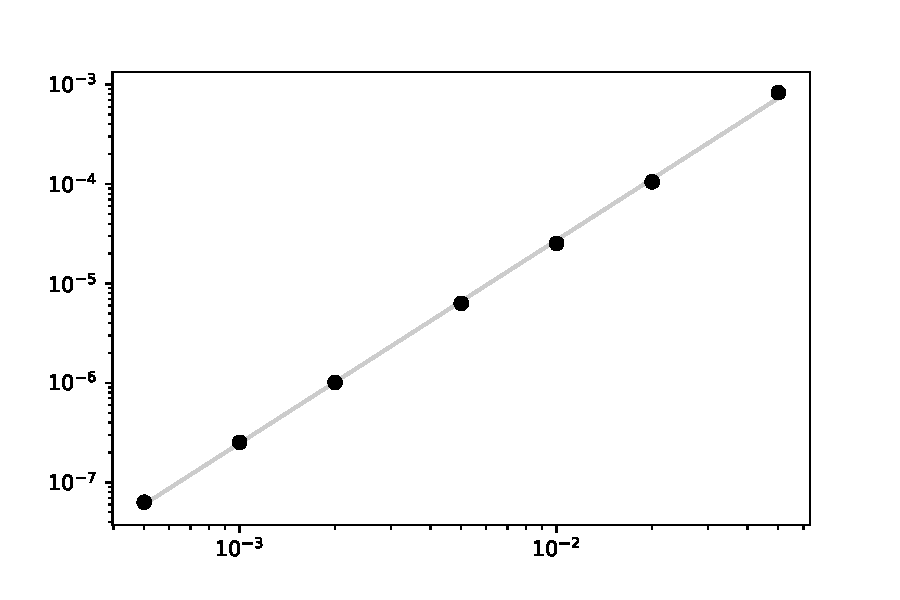
\includegraphics[width=\textwidth]{img/err.pdf}
        \caption{Trapezoid Rule}
        \label{trap}
    \end{subfigure}
    \begin{subfigure}{.32\textwidth}\centering
        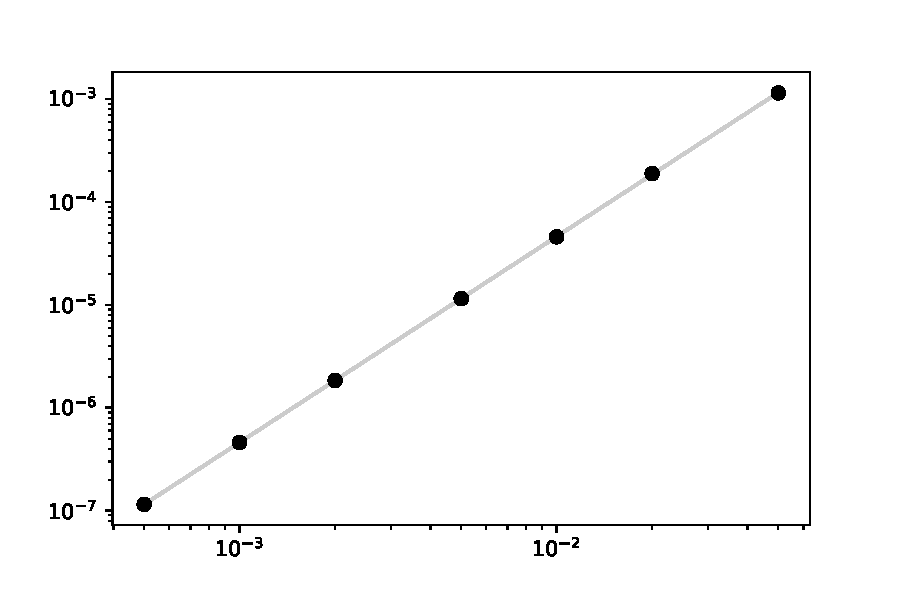
\includegraphics[width=\textwidth]{img/err_TRBDF2.pdf}
        \caption{TR-BDF2}
        \label{trbdf2}
    \end{subfigure}
    \begin{subfigure}{.32\textwidth}\centering
        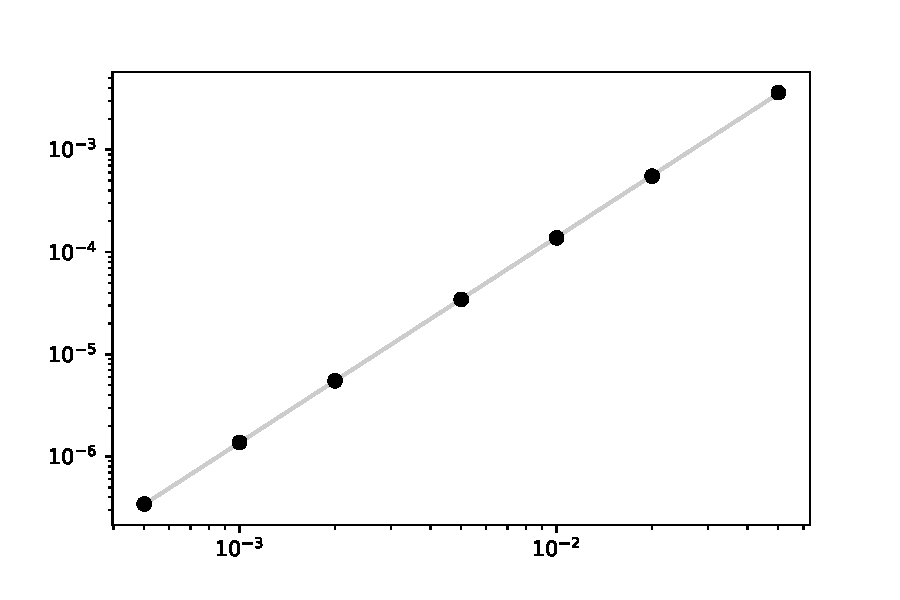
\includegraphics[width=\textwidth]{img/err_FWE.pdf}
        \caption{Forward Euler}
        \label{fwe}
    \end{subfigure}
    \caption{Infinity norm of error at \( T = 1 \) vs. mesh size \( h = 1/(m+1) \) when \( k=4h \). Linear fit to log-log plot shown in grey}
    \label{err}
    \end{figure}

    \item
    Our system is of the form,
    \begin{align*}
        U'(t) = f(U(t),t) = AU(t) + g(t)
    \end{align*}
    In particular we take \( A \) to be \( \kappa D_2 \) and \( g = (\kappa/h^2)[u(0,t), \ldots, u(1,t)]^T \).

    The TR-BDF2 method is defined as,
    \begin{align*}
        U^* &= U^n + \dfrac{k}{4}(f(U^n,t_n)+f(U^*,t_{n+1/2})) \\
        U^{n+1} &= \dfrac{1}{3} \left( 4U^* - U^n + kf(U^{n+1},t_{n+1}) \right)
    \end{align*}

    For our equations we have,
    \begin{align*}
        U^* &= U^n + \dfrac{k}{4}\left( AU^n + g_n + AU^* + g_* \right)
        && \Longrightarrow &&
        \left(I-\dfrac{k}{4}A\right)U^* = \left(I+\dfrac{k}{4}A\right)U^n + \dfrac{k}{4}\left( g_n+g_*) \right) \\
        U^{n+1} &= \dfrac{1}{3}\left( 4U^* - U^n + k(AU^{n+1}+g_{n+1}) \right)
        && \Longrightarrow &&
        \left( I-\dfrac{k}{3}A \right)U^{n+1} = \dfrac{1}{3}(4U^* - U^n) + \dfrac{k}{3}g_{n+1}
    \end{align*}

    We know that \( U^* \) represents a solution at time \( t_{n+1/2} = t_n+k/2 \). We implement this in Python and iterate over various mesh sizes to generate Figure~\ref{trbdf2}.


    Figure~\ref{err} shows a plot the infinity norm of the  error at (\( T = 1 \)). The slope of the log-log plot is \input{img/err_TRBDF2.txt} suggesting \( \cO(h^2) \) convergence when \( k=4h \).

    \item We have the same system as above. Using forward Euler we have,
    \begin{align*}
        U^{n+1} = U^{n} + k f(U^n) = U^n + kAU^n + kg_n
    \end{align*}

    We implement this in Python and iterate over various mesh sizes to generate Figure~\ref{fwe}.

    Note that the eigenvalues of \( A \) are,
    \begin{align*}
        \lambda_p = \dfrac{2\kappa}{h^2}(\cos(ph\pi)-1)
    \end{align*}

    Recall that forward Euler applied to the wave equation is stable provided,
    \begin{align*}
        \dfrac{k\kappa}{h^2} \leq \dfrac{1}{2}
    \end{align*}

    Clearly if \( \kappa = 1/50 \) and \( k=24h^2 \) this equation is satisfied.

    Figure~\ref{err} shows a plot the infinity norm of the  error at (\( T = 1 \)). The slope of the log-log plot is \input{img/err_FWE.txt} suggesting \( \cO(h^2) \) convergence when \( k=24h^2 \).

    \item
    If \( \kappa = 1/50 \) and \( k=26h^2 \) the condition for stability is not satisfied. We set \( k = 26h^2 \) and run to time \( T = 5 \) using \( m=39 \) interior mesh points. The solution is shown in Figure~\ref{unstable}. Clearly the solution is no longer converging as \( k\kappa/h^2 > 1/2 \).

    In particular,
    \begin{align*}
        |g(\xi)| = \left|1+2 \dfrac{k\kappa}{h^2}\cos(\xi h)-1)\right|
        = \left|1+ \dfrac{52}{50}(\cos(\xi h)-1)\right|
    \end{align*}
    will not be less than one in magnitude for \( \xi \notin (-\pi/h,\pi/h) \). This means that the method is unstable and we expect it to ``blow up'' at some point. Moreover, the \( \xi \) for which the method is unstable are the highest frequency modes of the DFT. This mode which alternates between 1 and -1 at each point explaining the alternating behavior in space seen in our solution.

    This behavior is not seen until a later time because the weight of eigenmodes corresponding to unstable \( \xi \) are small initially. More specifically, the modulus of the entries of the DFT of the Gaussian initial condition corresponding to high frequency modes are small initially . This means that it will take a while for these modes to blow up to a level which can be seen over the other stable modes.


    \begin{figure}[H]\centering
        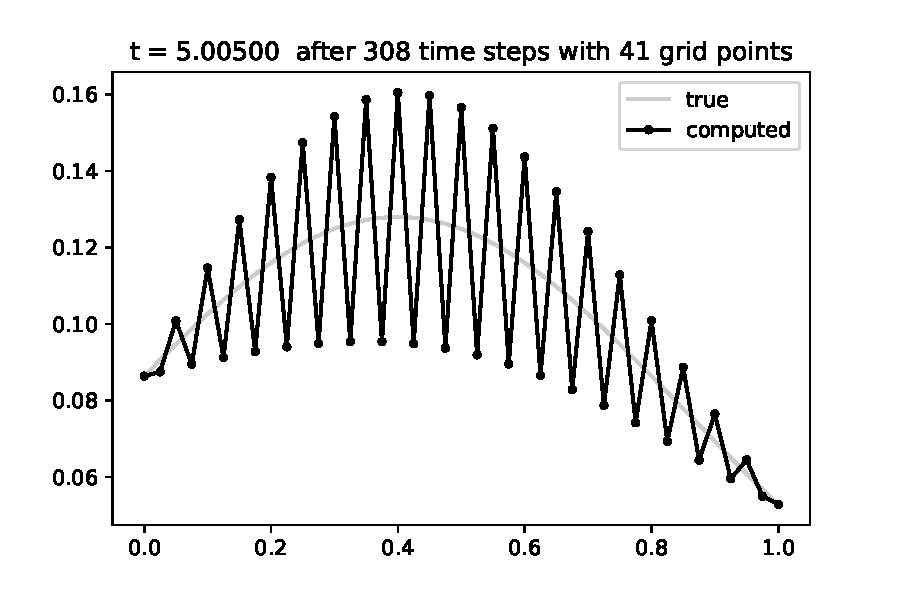
\includegraphics[width=.5\textwidth]{img/fwe_unstable.pdf}
        \caption{Solution using forward Euler with \( k=26h^2 \)}
    \label{unstable}
    \end{figure}

    \lstinputlisting[linerange=\#<start>-\#<end>]{heat_CN_TRBDF2.py}
    \lstinputlisting[linerange=\#<start>-\#<end>]{heat_CN_FWE.py}


\end{enumerate}
\end{solution}

\end{document}
